\documentclass{article}
\usepackage[utf8]{inputenc}
\usepackage{graphicx}
\usepackage{listings}
\usepackage{color}

\definecolor{dkgreen}{rgb}{0,0.6,0}
\definecolor{gray}{rgb}{0.5,0.5,0.5}
\definecolor{mauve}{rgb}{0.58,0,0.82}

\lstset{language=C,
  numbers=left,
  stepnumber=1,    
  firstnumber=1,
  numberfirstline=true
  aboveskip=5mm,
  belowskip=5mm,
  showstringspaces=false,
  columns=flexible,
  basicstyle={\small\ttfamily},
  numberstyle=\tiny\color{gray},
  keywordstyle=\color{blue},
  commentstyle=\color{dkgreen},
  stringstyle=\color{mauve},
  breaklines=true,
  breakatwhitespace=true
  tabsize=3
}

\title{Artificial Intelligence 1 \\ Lab 2}%Update the lab (assignment number)
\author{Bálint Hompot (s3177963) \& Ivo de Jong (s3174034) \\ AI1} %Change the names and fill in the student numbers and the group name (AI1/AI2/CS1 etc)
\date{19-05-2017}%Update the date

\begin{document}

\maketitle

\section*{Theory}
\subsection*{Exercise 1}
%Your answers for the theoretical questions go here


\textit{Run the algorithm several times, using different numbers of queens. Does the algorithm usually solve the problem?}

The perfomance is best for lower number of queens, starting from 4, which is the minimal number where a solution is possible. As the number of queens increases, so does the number of local optima, which decreases the chance of finding a solution.


\textit{In which situations does the algorithm not solve the problem. What can you do to improve the algorithm? Implement your suggestions for improvement.} 

The algorithm fails whenever the program gets stuck in a local optimum. A simple improvement to this could be random restart hill climbing, where on every iteration there is a chance for the computer to generate a random new begin state. We found that for 8 queens an optimum is usually found in less than 30 iteration. We'll make the chance fitting for this. We decided on a chance $p = 0.5$, which we found was decent through testing, and would go roughly one restart every 30 iterations. The performance on this is far better, as it's more like running 30 HillClimbs from different locations, and only one of them has to find a result.


\textit{Make a table and/or plot showing the success rate versus number of queens of your modified code}
%INSERT PLOT

The result shows that the performance is optimal for lower numbers. It should be noted that the percentage were determined on 100 tries per number of queens, so they are not entirely accurate, but they give a good indication.

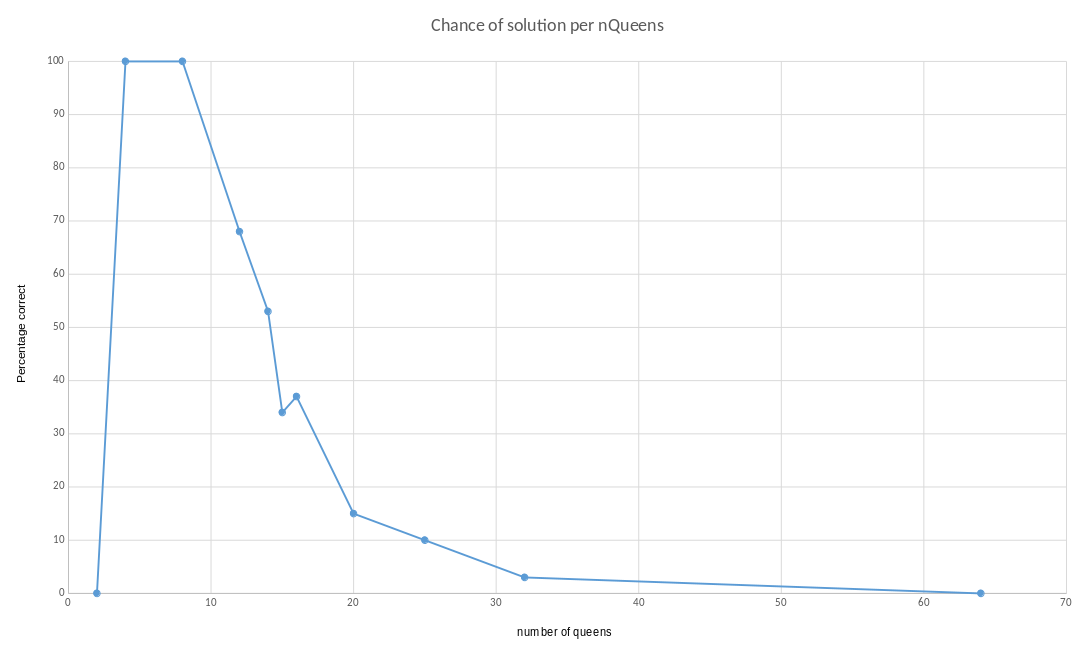
\includegraphics[scale=0.2]{./HillClimbGraph.png}

\subsection*{Exercise 2}
%Your answers for the theoretical questions go here


\textit{Define a suitable formula for the temperature as a function of time}

We decided that it would be best to distinguish between a linear function on time and a logarithmic one, as a logarithmic function is considerably better. The implemented logartihmic formula is $1.15^(dE / log(t))$, and the linear formula is $70^(dE/t)$. $dE$ represents the deviation the step makes, and $t$ represents the number of the iteration, ranging from 1 to 999.


\textit{ Run the algorithm using varying start temperatures and number of queens. Does the algorithm (often/always) return a solution? What settings should be chosen for which problem size?}

The algorithm is not very effective, as it seems to perform only slightly better than the original hill climb. This may be due to the probability functions being sub-optimal. We are seeing the general trend of allowing more mistakes at early iterations, but the plotting seems suboptimal. We know from the hillclimbing algorithm that there are many more local optima for larger number of queens, this means that more bad solutions should be allowed. This can be done by simpy increasing the constant in the formula, which is also a simple constant in the program.

\textit{Probably, your program does not work very well for problem sizes with more than 10 queens. Why is that? Try to modify your code, such that it also works for larger problem sizes. You may use any trick/heuristic that you can come up with, as long as the search remains a local search.}

Because there are a lot of local optima for larger number of queens, so it's easier to get stuck in the wrong optima. An easy fix would be to do random-restart hillclimbing. This should be done with a different formula from hill climbing, as there are more iterations for simulated annealing. Since simulated annealing needs more iterations we decided to not limit ourselves to the 1000 iterations given. This is also very doable as we don't consider as many possible states. We increase the number of iterations and decrease the chance to restart per iteration compared to hill climbing. The MAXITER is multiplied by 10 and the chance of restarting randomly is $\%1$.

\subsection*{Exercise 3}


\textit{Which of the three methods (Hill climbing, simulated annealing, and genetic algorithms) works best for the N-queens problem (for varying values of N)?}

We find that our genetic algorithm works best. It will often find a solution very quickly, even for very large boards. Moreover, the implementation is far more interesting. We find that for large numbers of queens even the genetic algorithm can get stuck in local optima. We could also add a random restart function to this, but we feel that this is excessive and that this would not appreciate the beauty of the genetic algorithm.


\section*{Programming nQueens} 
%The programming part follows the same template used during ADinC and Imperative Programming
\subsection*{Program description}
The program solves the nQueens problem with several search algorithms to find a solution. The nQueens problem is the problem where nQueens have to be placed on an n by n chessboard where none of the queens can threaten each other.
The performance is defined by $ (nqueens-1)*nqueens/2 -nConflicts$. This allows for an optimal performance $(nqueens-1)*nqueens/2$, where none of the queens are threatening eachother. This performance definition will be used in the problem solving algorithms. The fact that the global optimum is known allows us to easily stop the search when we found the global optimum. 

The first approach is the \verb!randomSearch! function, which generates a starting states and randomly shifts around queens. Needless to say the algorithm hardly ever finds a solution and is hardly usefull beyond academic value.

The second approach is the \verb!hillClimbing! function, which works similar to the \verb!randomSearch!, but will pick the best solution to move a queen to. This way the performance will always be increasing. This has been expanded with the option to random restart, to improve performance.

The third approach is the \verb!simulatedAnnealing! function, which also works similar to the \verb!randomSearch!, but will only let through bad moves with a chance p, based on the iteration and how bad the move is. Later iterations will have a smaller chance, and the worse the move, the smaller the chance. The weigth of the iteration can be done lineanly or logarithmically. This function also has an option to randomly restart.

The last approach implements a genetic algorithm approach for solving the problem. This takes a set of solution alternatives, and generates new generations of alternatives with breeding and mutating the previous generation until a solution is found.
\subsection*{Problem analysis}

The nQueen problem is defined as having a chessboard of n by n and placing n queens on it, where none of the queens can threaten eachother. There can be no possible solutions for $n<4$, and there are increasingly many solutions as n increases. The common version of this is the problem where $n=8$. It can be known that each column will only have one queen, which somewhat simplifies the problem. This gives that for 8 queens there are $8! = 40320$ tries to be done to generate every solution. (This has the implicaiton where 2 queens can't be on the same row either.) This is already quite a few, but it's not hard to see that as n increases, the amount of solutions increases exponetially. The general approach our functions use is randomly generating a state with 1 queen per column, and making movements where the performance is improved. The performance decreases as more queens threaten eachother. This way the program could find an optimal solution in just a few steps. However, there are a lot of \textit{local optima} where the performance is not optimal, but the performance can't be improved by moving only one piece. This is where randomly restarting allows the program to search for another optimum. The genetic algortithm and simulated annealing allow for taking steps back with chance to still find the optimal solution. Since the global optimal performance is known an implementation could be made where the program keeps restarting until the goal performance is found, but we felt that this could take too long and holds no academic value.

\subsection*{Program design}
We will not go into the program design for the \verb!randomSearch! function as it is not our work and it is too simple.

The queens are represented in an array of size $n$, where each slot in the array contains an integer to represent in which row the queen is. This is easier for some of the operation and doesn't allocate unnecessary memory. The given program gives this as a global, and the function to calculate the performance is therefore also applied to this global array. The program will stop once a maximum number of iterations is reached or the goal performance is found. 

For hill climbing a random queen is picked and iteratively moved to every other row. The performance is measured after each movement and placed in an array where the index defines the row, and the value gives the performance. This has te be done in this way since the performance function only operates on the global array. After this, the index with the best performance is chosen and the queen is moved to this location. This way very few iterations have to be made to find a local optimum. To battle the problem of getting stuck in a local optimum we added a random restart option, where on every iteration there is a $\%5$ chance of restarting with a random state. Over the 1000 given iterations it will generally restart about 30-50 times, which significantly improves performance. 

The simulated annealing is done similarly to the hill climbing, except the program does not find the best row for a queen, but choses a random row. If the new state is better the program reiterates. If the new state is worse a function of chance is called. This function gives a chance to keep the queen or move it back. The probability for this is $1.15^(dE / log(t))$, or $70^(dE/t)$. Here dE represents the deviation from the previous state and t the iteration. Either formula can be chosen by the operator to find whether a linear or logarithmic approach is better. We chose for different constants to compensate for the effect that the log operation has on the chance. The variable were found through testing the program with various values. These values seem decent, but could be perfected by extensive testing. The probability was made from the formula $e^(dE/T)$, which is the standard formula for simulated annealing. For the simulated annealing we also implemented an option to randomly restart, but with a much smaller chance of $\%1$, as the simulated annealing needs more small iterations to reach an optimum. To accomodate for this the maximum number of iterations is also multiplied by 10. The iterations take less processing $O(1)$ than the hill climbing does $O(n)$, so it is justified.

The genetic algorithm introduces new variables: an individual looks like the global nqueens array, but this time we need several of this kind. Therefore we introduce two arrays for storing the current and the next generation, both containing 100 individuals. We also introduced a simple int array for storing the individual fitness values for inserting them in order. This could have been done with defining a generation struct as well. We also introduced son1 and son2 variables, to use them when generating new individuals.\\
The algorithm works as follows: it generates two sons from the current generation, and inserts them in order of their fitness (number of conflicts) to the next generation array, until it is filled with 100 individual, which seemed an optimal number in our runs. For that an insertInOrder function was defined, that inserts the son to the correct place and shifts everything after that (a heap could be used, but not crucial in this task), and a conflict counter, which is the same as the one used for the other solutions, but it takes an individual as an argument, instead of the global nqueens individual. Then the current array is updated to the next, the global individual is updated to the best from the next generation, and the loop starts again, until a solution is found, or the generation limit is extended.
Generating the new individualsrelies on the function newIndividual. It takes the current generation, and the son arrays, because the generated individuals will be stored in them. Since the genom of an indiviual is a column number for each row, the genom could be easily cut an any point, and stuck together for the new individuals to create a valid son. This is the method we used for crossover. The parents are chosen randomly, with the ones in the beginning having a greater chance to be chosen: the index of the individual is subtracted from the population size, divided by 3, and then checked if it is greater than a random number between 0 and the population size divided by 2. This method gives a linearly decreasing probability, that is not too steeply decreasing, and does not start from a too high chance for the best individiuals. The two parents must be different individuals.
We also implemented a simple mutation method: since swapping the value of a row creates a valid individual (if the new value is within the size of the table), we could use this method for more variability and to avoid local optima.


\subsection*{Program evaluation}
The program takes very little memory because it uses local search. The computations needed also isn't very much as it doesn't scale exponentially like brute force would. Because the program doesn't dynamically allocate memory we won't include a valgrind report, as there can't be any leaks.

The hill climbing allocates memory in order O(n), but since this is limited in the input, the memory is simply allocated as maximal. The processing is a bit heavy as for every queen that is picked, all slots are considered. The biggest weight in the processing effort is simply in the maximum number of iterations, which is quite low when the global optimum is found. Sadly,the program does not always find a solution, specifically for $n>12$. This is of course the most limiting factor for this program. A graph of this can be found below. The graph shows that it can (almost) always find a solution for smaller number of queens, but when there are too many queens it won't find a solution within the number of iterations. If the number of iterations is removed it will always find a limit, but this can take a very long, which is why we did keep it limited.
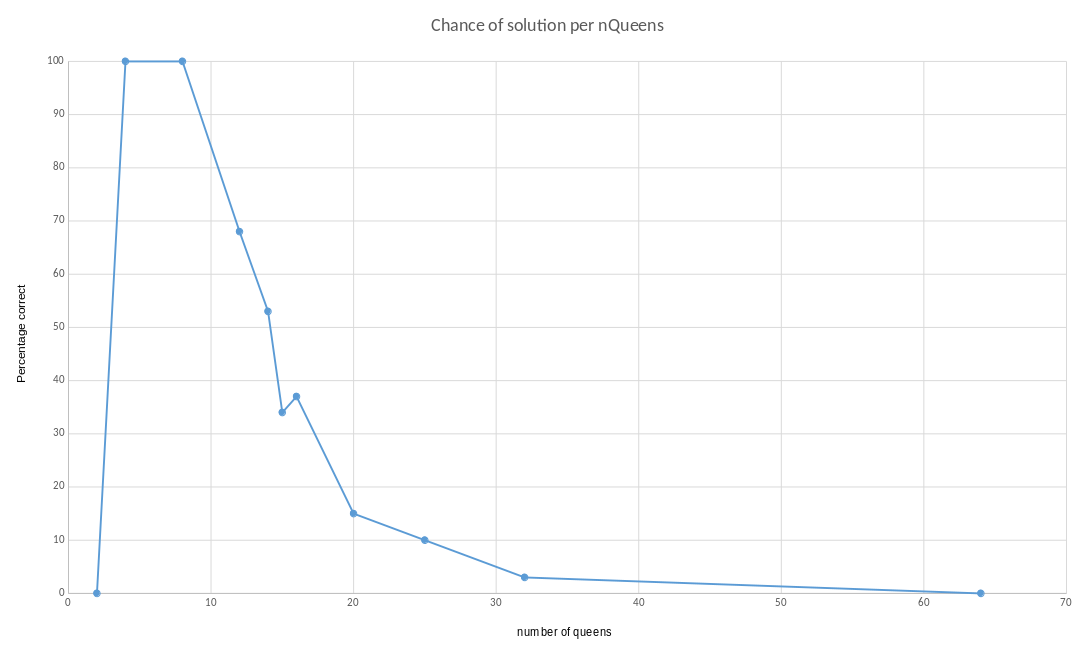
\includegraphics[scale=0.2]{./HillClimbGraph.png}

The simulated annealing doesn't allocate the memory like in hill climbing, as it only takes single steps. The processing per iteration is a lot less, since a random move is performed instead of the best move. However it ultimately does take more processing as the maximum number of iterations is multiplied by 10. The simulated annealing is more likely to find a solution than the hill climbing, but it still has issues when then number of queens is larger. It works better than hill climbing both with and without random restart. The logarithmic formula appears to perform slightly better than the linear one, but the difference is slim. 

The genetic algorithm however works very efficiently for this problem: even for bigger table sizes, like 20 - 40 it is able to find the solution normally in a couple hundred generations. For smaller sizes it usually find in less than 100 generations. Even for states between 40 and 65 the solution is found in a couple of thousand generations. Above that, the solution becomes really complex, and the program seems to get stuck with local optima: this could be prevented by higher mutation ratio, or more chance for the less fit individuals to breed, but that could lower the effectiveness for smaller tables. 

\subsection*{Program output}
The program starts with a simple dialogue where the user selects an algorithm, and for some give details regarding the algorithm. The initial state is always randomly generated and presented to the user, as it might be interesting to see which states allow for solutions. A queen is presented with a lower case q or upper case Q, where the upper case represents a threatened queen and lower case represents a safe queen. 

During the algorithm, every algorithm presents the iteration and performance, except the genetic algortithm, which shows the generation and fitness. This allows the user to see how the state is improving. 
For simulated annealing and hillclimbing every movement is shown so every intermediate state could be calculated from the output. Simulated annealing also shows the chance to pass bad values (and the generated number), so the pattern of the temperature is visible. At the end they both show the number of random restarts, and simulated annealing also shows how many bad moves are let through. 

The program always ends with the final state as explained before. This can either be a solved board, (indicated by "Sovled puzzle") or an unsolved board.

\subsection*{Program files}
%copy code files into listings using the \begin{listing} command as follows:
\subsubsection*{nQueens.c}
\lstinputlisting{nqueens.c}

\section*{Programming Nim} 
%The programming part follows the same template used during ADinC and Imperative Programming
\subsection*{Program description}
The task was to implement an effective solution for the game of nim. This is the game, where the players can pick 1,2, or 3 matchsticks from a set, and whoever picks the last one loses. The solution is based on the minimax algorithm, that calculates the final outcomes for all possible moves, and chooses the optimal one.\\
For example for 3 or 4 matsticks, the starting player has a direct option to win the game, taking 2 and 3 sticks, and force the other player to take the last one. These branches would be evaluated for 1, and the minimax would choose these branches.\\
On the other hand, for 5 sticks no matter what the first player does, the second has an option to win (3->1, 2->2, 1->3), so all branches would worth -1, and the starting player looses in all cases. For 6 sticks however, the starter has an option to reduce the state to 5, forcing the second player to loose, as they would be in the situation described above. In this case, the move 1 would lead to the value 1, and the other moves would lead to the value -1, so the move 1 would be chosen.
\subsection*{Problem analysis}
A version of minimax algorithm for the problem was given, but it was using separate min and max functions, and double function calls with one returning the value of the minimax, and the other returning the move. Our task was to implement a negamax function for the problem, that returns both. The task was also to implement a transposition table, that stores the optimal choice for players at states, so there would br no need to calculate the same moves over and over again. This is especially useful in this game, since many paths lead to repeating states, and both players are playing optimally, so they would take the path that was calculated during the first step.

\subsection*{Program design}
To solve the problem of different return types, we introduced a new struct called Choice, that contains both the value and the move. We defined our negaMax function to return this type. The negaMax is based on minimaxDecision, but it makes the difference between MAX and MIN turns with the turn value, which is 1 (MAX) or -1 (MIN). Whenever a calculation takes place, the correct variables are multiplied by the turn variable (f.e.: the return value is initially infinity, and it is always checked if smaller than turn times the returned value from the recursive call), and the return value at leafs also depends on the turn variable. Whenever the negaMax is called recursively, the turn value is multiplied by -1, to suit the calcuations for the player in the next turn. With this recursive function, returning a Choice we could also avoid to use two different functions in different depths, like minimaxDecision and minValue in the original solution, because every step and value can be calcuated with a simple recursive call. We also implemented a simple user input to choose between the classic (original) and the negaMax vesion, to make the comparison easier. The classic solution was not change at all. \\
Before implementing the transposition table, we also included two minor modifications for the negamax algorithm, that are really simple, but make the program a lot more effective than the original solution. The first was to evaluate the moves in decreasing order: this way, if there are branches with the same value, the biggest step is chosen, resulting in a shorter sequence and faster solution time. The second was to stop looking for other branches if an optimal value (e.g.1 for MAX) has already been found. This is possible, since there are no difference between branch ends, just the value 1 and -1.\\
The transposition table was designed to store the values for MAX and MIN for the states that have already been evaluated. The implementation is a matrix of Choice structs, that has one dimension for the states (sticks left), and a dimension for the player. (MAX or MIN). In the beginning of every negaMax call, the table is checked, if a value exists for the state and player. If not, the choice is calculated and stored. At the end the function retrieves the value from the table (no matter it is newly stored or not). The table has 101 states, because the state numbering starts from 1, and not from 0, as it is in an array, so a state of 100 sticks needs a [100] index.
\subsection*{Program evaluation}
When using the classic version, or the negamax version before the efficiency enhancements were implemented, the program fast for sets of 10 and 20, but it slowed down for states above 30, for states around 40 or more it was too slow for us to wait for an output. It was also interesting to see how the exponential growth of branches shows in this task: for the state of 35 for example, the first step takes a long time, the second takes a lot shorter, but still noticable, and the rest is calculated within a second.\\
After implementing the two tricks, but before the transposition table the efficiency improved significantly: the program was able to calculate the output up to 80 sticks in a couple of seconds. The output showed a different sequence then in the classic method, because of the order changing, but that is not a problem, since there are multiple optimal paths for winning.
The transposition table gave an other significant improvement for the program: after the implementation the program was able to produce the correct output for even the maximal 100 matchsticks within a second, the set of 50 sticks meant no problem for a very fast output.

\subsection*{Program output}
The program outputs the sequence of steps for the best outcome for MAX, the first player. For all cases where the starting state is not 5 the game is winnable for MAX. Moreover, the program prints the shortest optimal path for MAX, taking the most sticks whenever multiple equally good solutions are possible. For the negaMax solution it also prints out the evaluation of the taken path.

\subsection*{Program files}
%copy code files into listings using the \begin{listing} command as follows:
\subsubsection*{nim.c}
\lstinputlisting{./nim.c}

\end{document}